\chapter{\textbf{Queueing Network Solving And BottleNeckAnaliysis}}

Once parameterized the Queueing Network, the data was inserted into Java Modelling Tool (JMT). It was decided to carry out a simulation with a number of SeaweedPickingInland/Outgiung equal to one thousand for each.\\
Various output Indices were analyzed in first analysis. Performance Indices:
\begin{itemize}
\item Utilization:
	\begin{itemize}
		\item Control Center Server;
		\item SeaweedPicking Control Unit;
		\item Water Company Server;
		\item Purification System;
		\item Water Company Disk.
	\end{itemize}
\item Response Time:
	\begin{itemize}
		\item Control Center Server;
		\item SeaweedPicking Control Unit;
		\item Water Company Server;
		\item Purification System;
		\item Water Company Disk.
	\end{itemize}
\item Response Time Sink (Check Water Quality);
\item Throughput for Sink (Check Water Quality).
\end{itemize}

\begin{center}
  \makebox[\textwidth]{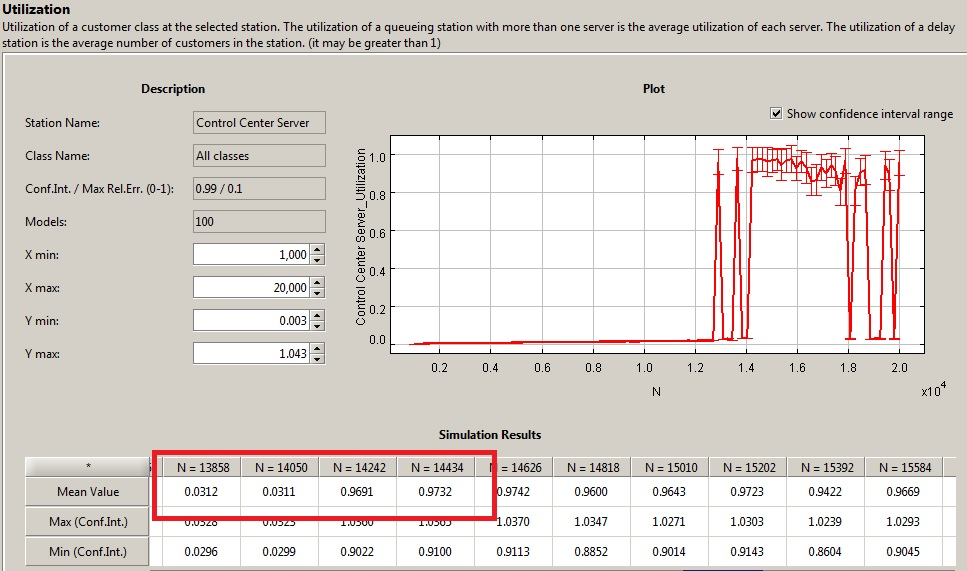
\includegraphics[width=\textwidth]
 {1-UtilizationControlCenterServer.jpg}}
\end{center}
\captionof{figure}{Control Center Server Utilization}

\begin{center}
  \makebox[\textwidth]{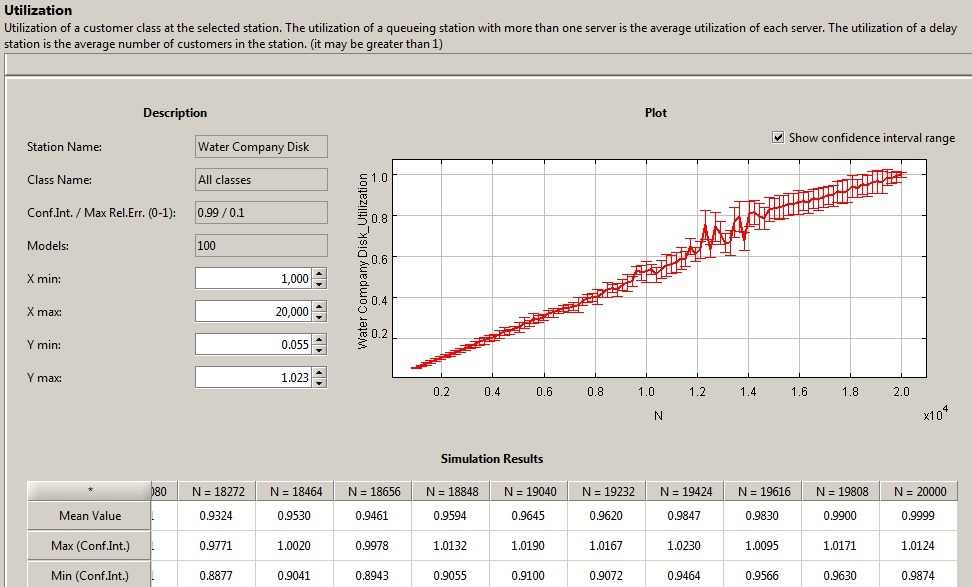
\includegraphics[width=\textwidth]
 {2-UtilizationWaterCompanyDisk.jpg}}
\end{center}
\captionof{figure}{Water Company Disk Utilization}
\bigskip

It resulted that the simulation was successful for all performance
indices. Then we choose to run multiple simulations with increasing
number of sensors to understand how the system scales and how it
respond to the increasing of inputs. For this purpose we have done a What-If simulation composed of one hundred sub-simulation and it has come out that the Utilization performance of the Control Center Server, Water Company Disk gets worse when the fourteen thousand sensors are reached.\\
Other proof of this is the analysis of the Response Time.

\section{Refactoring}

For the refactoring phase we wanted to consider the case in which we want to increase the number of Seaweed Picking to twenty thousand units. in this case, as we saw in the previous analysis, we have a bottleneck linked to the Control Center Server and to the Water Company Disk.

\begin{itemize}
	\item Software Solution;
	\item Hardware Solution.
\end{itemize}

We have chosen a hybrid solution because we have halved the service time for each class of jobs for the Water Company Disk and for the Control Center Server, and decided to have two separate Water Company Disks one for the Sample Inland and one for the Sample Outgoing that translates into a modification of the architecture.\\
In addition, by resolving the new model we noticed an unexpected increase in the use of SCPU and for this reason we have slightly reduced the service time of this node. The results are shown below:

\bigskip
\begin{center}
  \makebox[\textwidth]{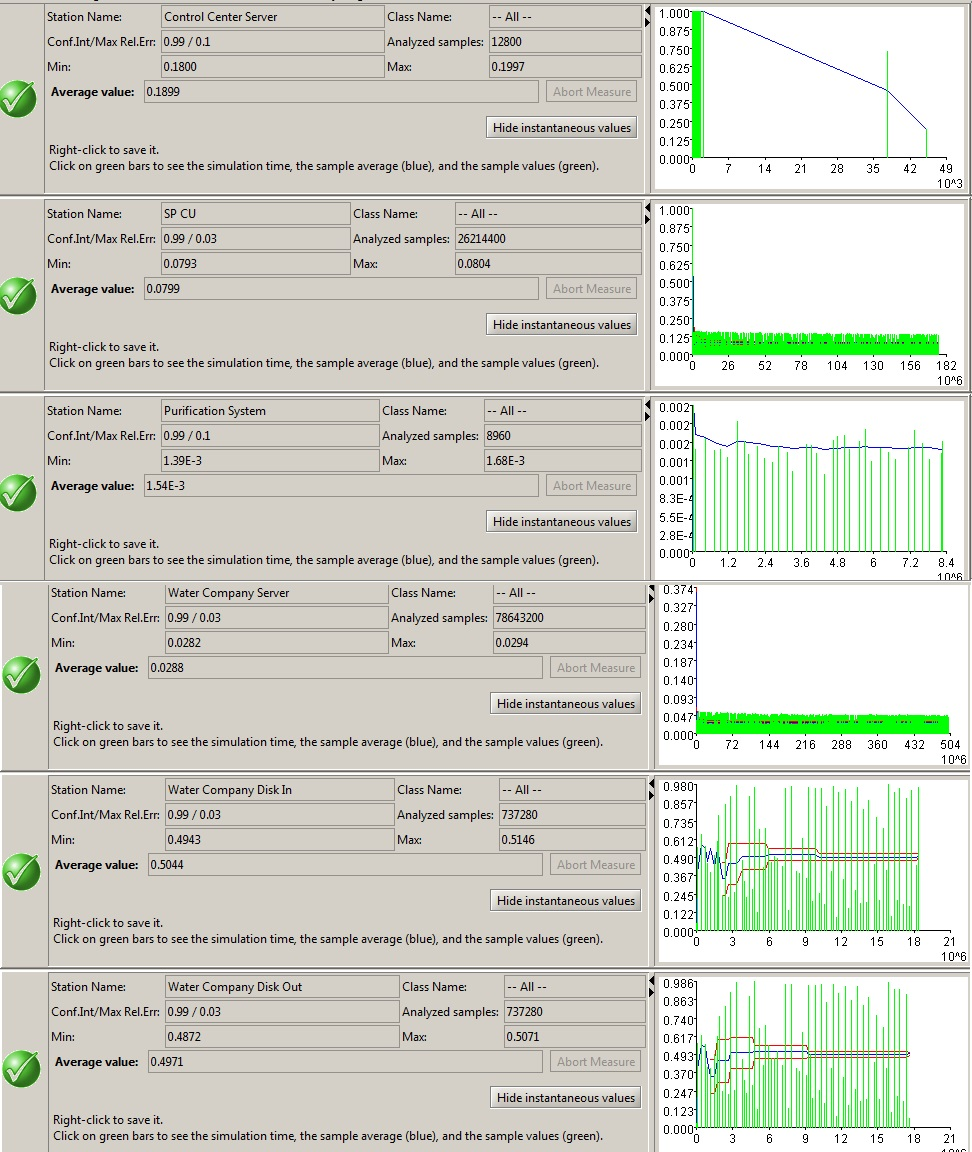
\includegraphics[width=12cm]
 {3-UtilizationRefactoring.jpg}}
\end{center}
\captionof{figure}{Utilization Refactoring}